\chapter*{Introdução}\label{introducao}
\pagestyle{introducao}

O debate e as reflexões sobre a imagem, como ela é construída e se
apresenta no mundo atual, estão cada vez mais presentes em muitos
campos de investigação. A escolha de um ponto de vista para se falar
sobre um assunto tão amplamente discutido, não é uma tarefa fácil. Um
dos problemas mais comuns, para aqueles que decidem mergulhar no
complexo mundo da pintura, é decidir de que forma a tela branca será
abordada para expressar aquilo que, por hipótese, seria uma
representação de suas ideias. A distância entre o suporte e a mão do
artista é aparentemente curta, mas existe um longo percurso, que tem
sido descrito pela história da pintura ocidental, até que a obra seja
considerada acabada e apta a enfrentar o olhar do outro. Além disto,
cada vez mais pessoas, cujo repertório visual não necessariamente se
relaciona ao mundo da pintura, demonstram interesse em se iniciar no
mundo das artes visuais. No sentido inverso,
\textcquote[131]{sabino2000pintura}{muitos artistas possuem uma vontade
	criativa, em determinado momento de seu percurso, de usar suportes e
	meios de expressão exteriores ao da própria pintura}

O caminho para a busca do autoconhecimento e a consequente seleção de
meus principais interesses de investigação foram estratégias decisivas
para dar clareza a questionamentos para os quais não tinha respostas. A
lembrança do fazer experimental, por meio de uma câmera de filme Super
8, durante a graduação em cinema nos anos 1980 abriu espaço para as
questões que permanecem até hoje, que se resumem ao problema do olhar
mediado ou não por um dispositivo.

A presente dissertação é o resultado de uma investigação durante o
curso de mestrado em artes plásticas da Faculdade de Belas Artes da
Universidade do Porto e, principalmente, da minha busca pessoal,
enquanto artista/investigadora, por delimitar um dos campos de pesquisa
que considero mais importantes no exercício da atividade do pintor, que
é a construção de uma imagem. As reflexões sobre a prática em ateliê,
aprofundadas ao longo do período de estudos deste mestrado, trouxeram à
tona as seguintes indagações teórico-práticas recorrentes, que já se
apresentavam muitos anos antes do início do curso:

\begin{itemize}
	\item Qual a possibilidade de se utilizar o olhar característico do cinema,
	      no método processual da construção de uma pintura?

	\item Como se movimentam os olhos dos espectadores diante de uma pintura?

	\item Como é feita a seleção, pelos pintores, das referências que apoiarão
	      seus projetos?
\end{itemize}
\noindent E, na busca de compreender e lidar com estes dois universos do meu
percurso pessoal, passei a investigar as possíveis relações da pintura
com o cinema e do cinema com a pintura.

\begin{figure}[t]
  \caption{\artname{\odette}{Ando}{2012}}

	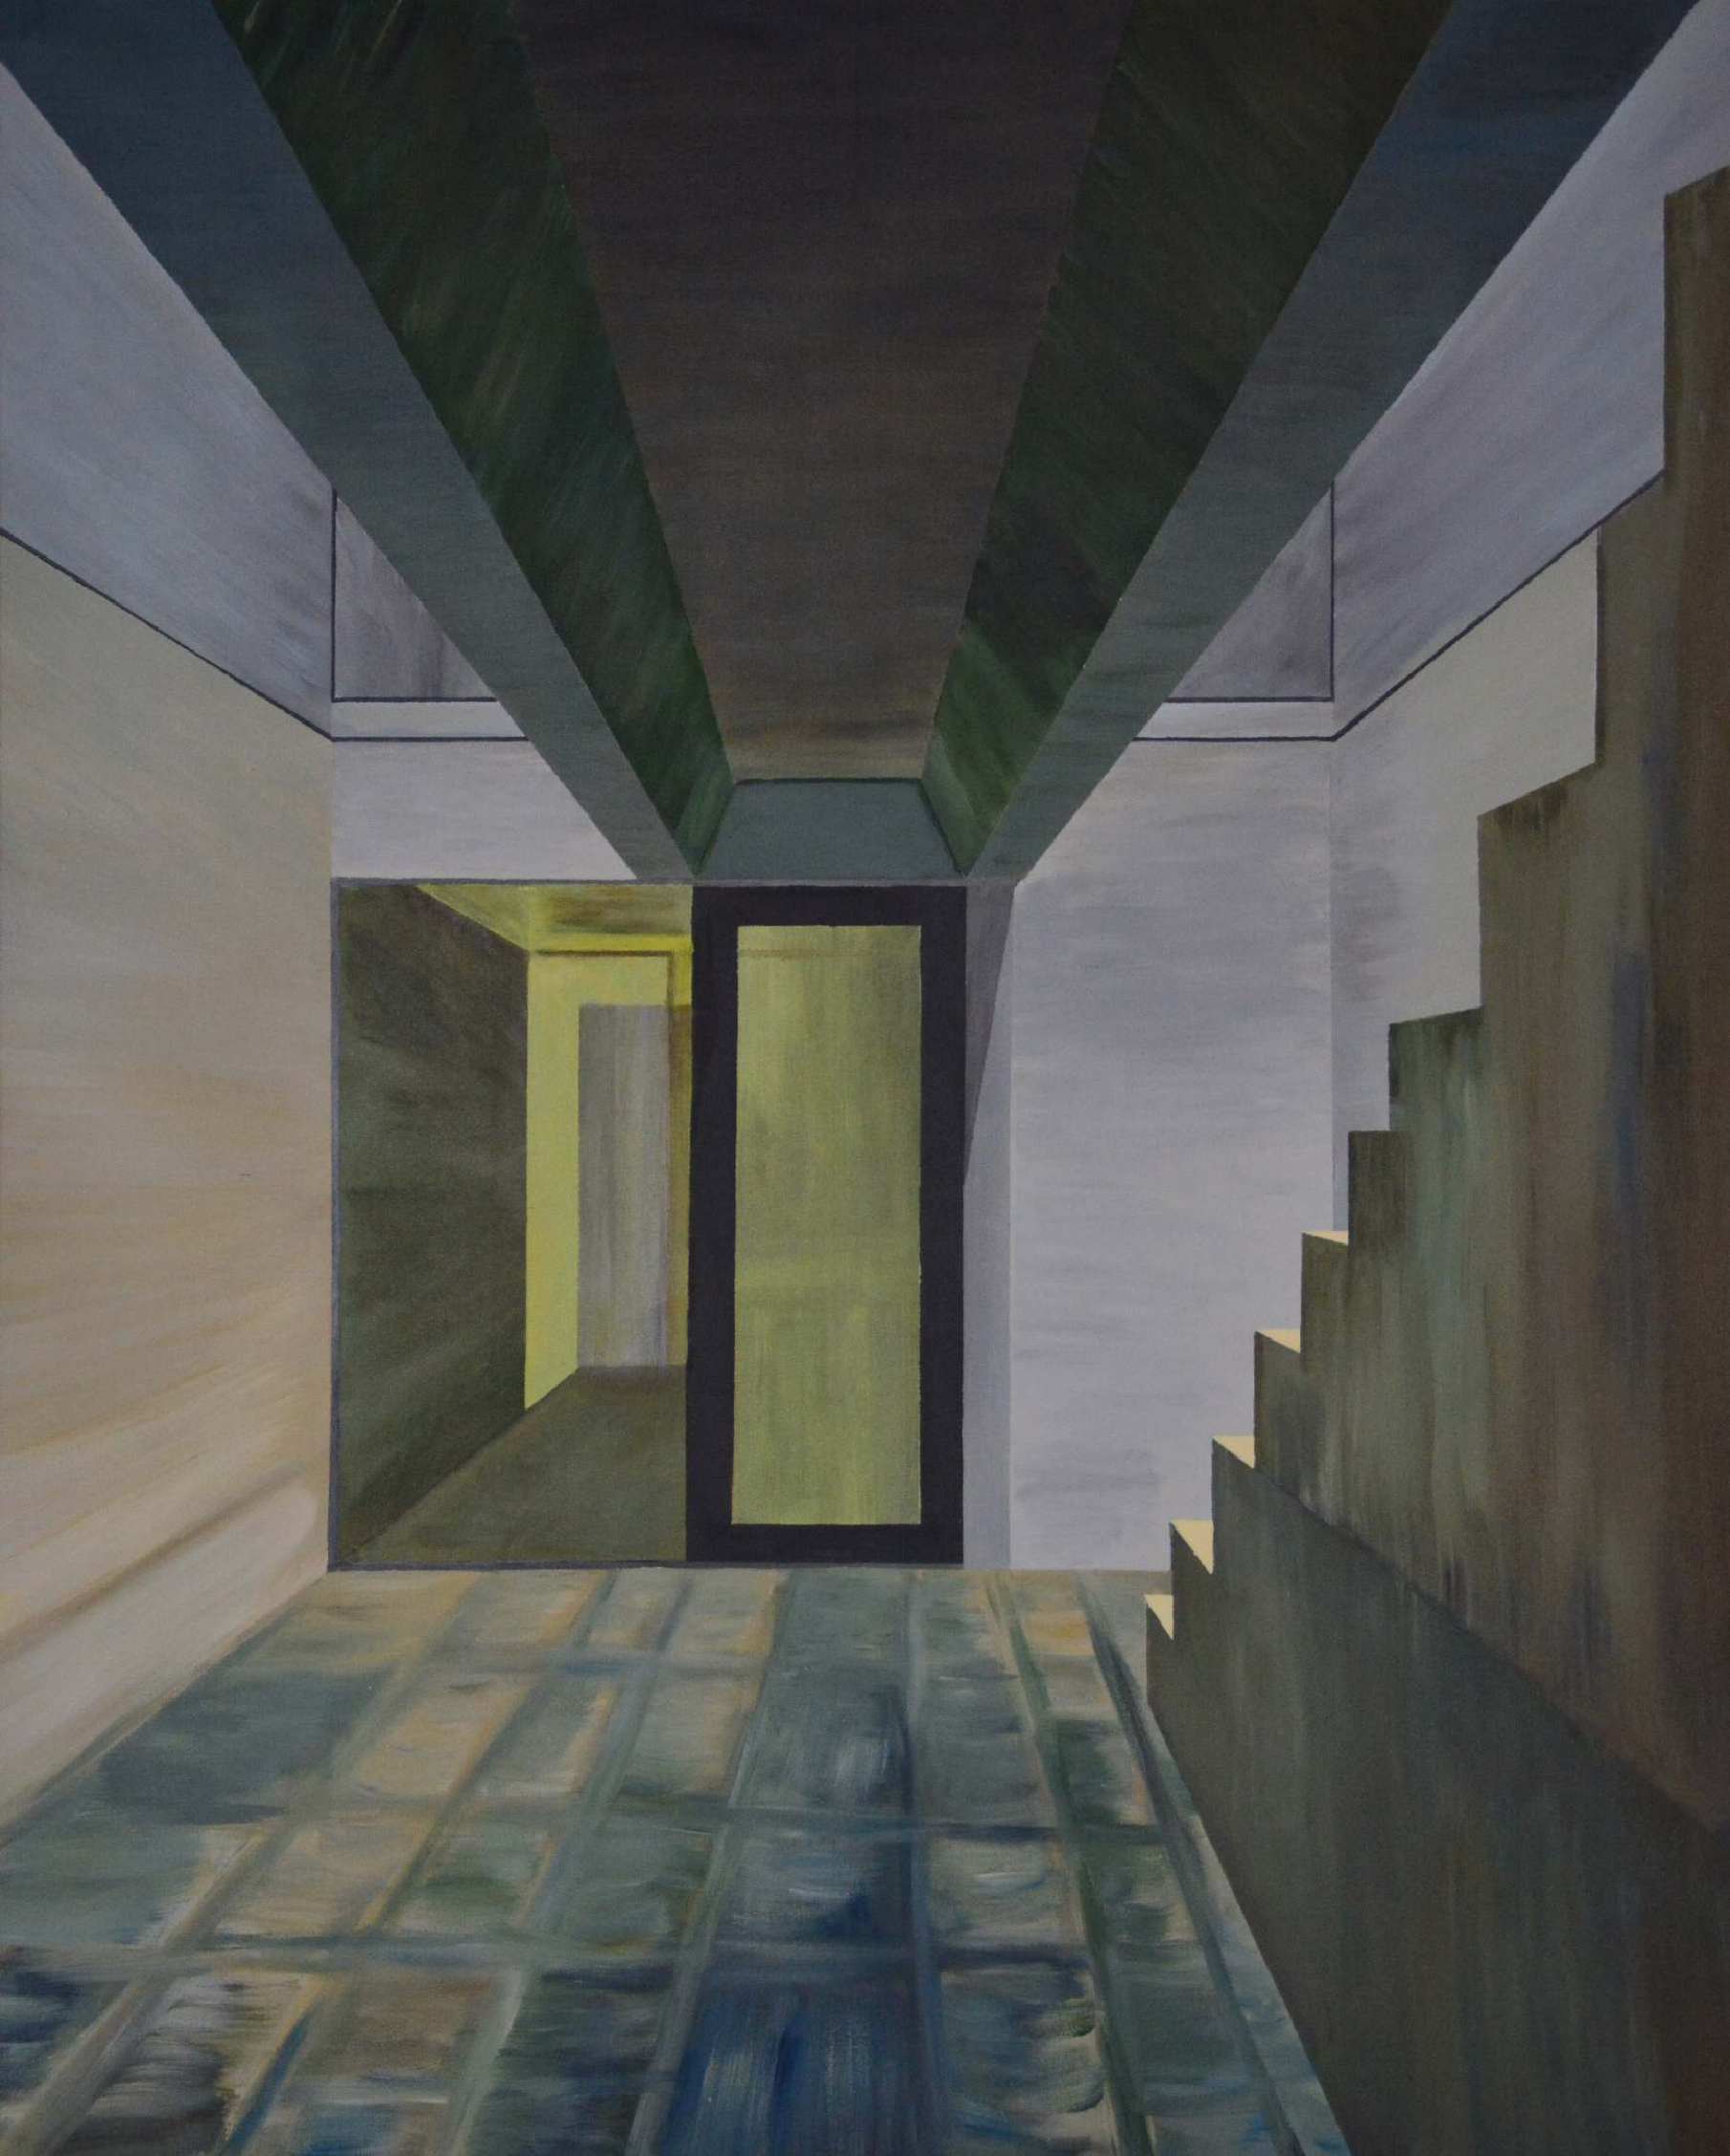
\includegraphics[width=2.8in]{odette-ando-2012.pdf.compressed.pdf}
  \figurenote{\series{Construir}. \oleo. \artsize{104 x 97}.}
\end{figure}

Meu interesse pela construção da imagem na pintura surge na Escola de
Artes Visuais do Parque Lage, no Rio de Janeiro, a partir de 2011,
quando tive o primeiro contato com o estudo prático de pintura, onde o
foco principal era a pintura contemporânea. Participei de vários cursos
livres, marcados pela didática de professores pintores que integraram o
grupo \emph{Como vai você Geraçāo 80.} Conforme aponta
\textcite{bulhoes2018geracao}, a maioria dos artistas que faziam parte
desta geração nasceu após o fim da Segunda Guerra Mundial, em meio à
guerra fria, e se nutriam da indústria cultural norte americana que
entrava no Brasil durante os anos 1970. A televisão, o cinema, as
revistas em quadrinhos e os super-heróis eram a sua base imagética,
sem, no entanto, configurar um grupo ou movimento artístico
ideologicamente coeso. Após cerca de 10 anos de predomínio da arte
conceitual, a produção local ecoava a Transvanguarda italiana, a
\emph{Bad painting} norte-americana e o Neoexpressionismo alemão \parencite[62]{bulhoes2018geracao}. Uma das características dos trabalhos
deste grupo era a grande dimensão~das telas, quase sempre livre dos
chassis, o que proporcionava gestos pictóricos com maior decisão, além
da maior liberdade do uso das cores. Em 2011, o ensino na EAV era
fortemente pautado em processos artísticos, que naturalmente
amadureceriam as poéticas pessoais dos alunos, a partir do fazer. O
acompanhamento dos professores/artistas se dava com uma mínima
interferência, com o apoio ao desenvolvimento dos estudantes, partindo
de seus próprios interesses. Nos apresentavam técnicas de artistas
contemporâneos, tanto brasileiros quanto internacionais, com múltiplas
possibilidades de processos em suas poéticas. Publicações como
\emph{Vitamin P} e livros específicos de pintores que faziam sucesso em
feiras de arte internacionais deixavam difícil a escolha pelo caminho a
trilhar. Vivíamos entre imagens que chegavam pelos livros de Eric
Fischl, Lucian Freud, Luc Tuymans, Michael Borremans e Jenny Saville,
além dos brasileiros que nos rodeavam, entre eles Luiz Zerbini, Daniel
Senise, Adriana Varejāo, Lucia Laguna, Cristina Canale e o próprio Luiz
Ernesto, um dos nossos professores. Diante de tantas possibilidades,
naquele momento, me sentia intrigada e queria compreender como é feita
a seleção pelos pintores das referências que apoiarão seus projetos,
sendo esta uma das questões presentes nesta investigação. Fui
incentivada a realizar pinturas em grandes formatos, com tinta
acrílica, tendo como modelo fotografias que eu mesma tirava.
Entretanto, o que eu precisava saber era como construir uma imagem
diretamente no espaço de uma tela de pintura, uma vez que as
experiências anteriores com a visualidade foram mediadas por uma câmera
de fotografia ou uma filmadora. Segundo \textcite{sabino2000pintura},
no cinema há muitas vezes a contaminação da
pintura, não só pela sua expressão, mas também pelo olhar pictórico. O
modelo pictural, de algum modo, colabora noutros processos criativos.
Por outro lado, poderemos pensar numa ampliação e reformulação do
próprio conceito de pintura um pouco como se adquirisse, por osmose e
mutação características híbridas, pilhadas de outros territórios 
\parencite[132-133]{sabino2000pintura}.

Mas o que poderíamos chamar de um olhar característico da atividade
cinematográfica? Em uma prática com o audiovisual, anterior à pintura,
o dispositivo que se instalava entre o olhar, o objeto e a imagem
sensibilizada, realizava rapidamente aproximações e afastamentos que
traziam o detalhe para bem perto, ou para longe, ao reestruturar os
enquadramentos, ângulos e pontos de vista. A minha graduação em cinema,
nos anos 80, deixou ecos de teorias sobre planos próximos, médios e
grandes planos, e também sobre movimentos de câmera, que naquele
momento na EAV precisavam se conectar a um mundo de denominações, até
então desconhecidas, e uma longa história da pintura, ainda por serem
desvendadas. O desafio, então, era estabelecer o formato inicial da
pintura, com proporções e regras bem diferentes das que eu estava
habituada. As fotografias de referência de espaços arquitetónicos
contemporâneos, retiradas de revistas, contribuíam para iniciar alguns
estudos sobre perspectiva.

\begin{figure}[h]
  \flushright
  \begin{minipage}{3.45869in}
  \caption{\artname{Odette Boudet}{Processo da pintura Cávea}{2014}}

	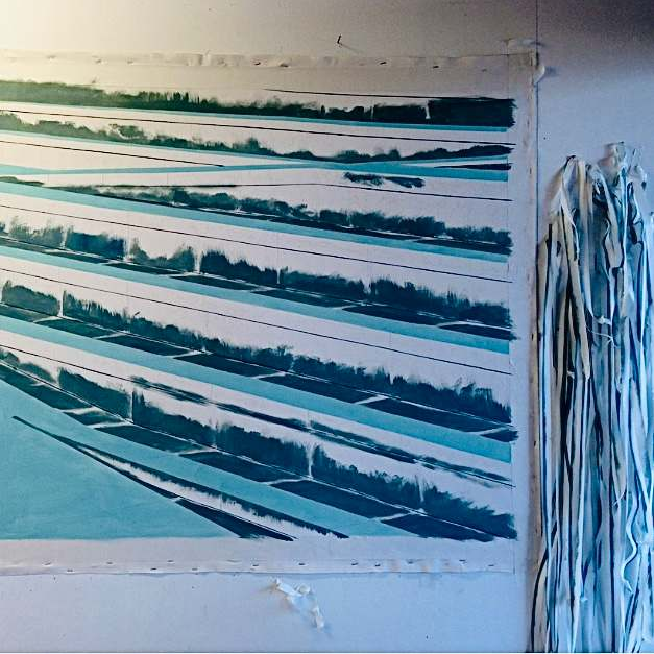
\includegraphics[width=3in]{figuras/odette-processo-pintura-cavea-2014.pdf.compressed.pdf}
  \figurenote{\series{Arena}. \acrilico. \artsize{104 x 97}. \photoreg.}
\end{minipage}
\end{figure}

No meu processo, marcava as linhas estruturais retas usando tinta e
fita crepe diretamente sobre a tela, realizando a medição de pontos de
fuga com cordas e barbantes.


Em 2016, já trabalhando em ateliê próprio, busquei um aperfeiçoamento
na pintura a óleo e também conhecer o passado histórico através da
Escola de Belas Artes --- \ac{ufrj}. Por meio de autores como
\textcite{wolfflin2000conceitos,argan2010arte,itten1975arte}, iniciei
um estudo teórico das artes, com ênfase em conceitos da visualidade,
trabalhados ao longo da história da pintura. Aos estudos experimentais
de perspectiva, somaram-se histórias dos primórdios matemáticos
geométricos das \emph{golden lines}, que remontavam ao período
renascentista da pintura.\newpage

Este exercício de revisitar os principais interesses pessoais e estudos
relacionados aos problemas do olhar \emph{despoletou}\footnote{In
	priberan \enquote{fazer surgir ou desencadear} (ex.:~\emph{despoletar
		comportamentos preventivos}). Este último uso é bastante generalizado,
	mas contestado por alguns autores, que alegam tratar-se de um emprego
	contrário ao sentido original da palavra. Uma vez que
	a~\hiperlink{https://dicionario.priberam.org/espoleta}{espoleta}~é peça que
	desencadeia a explosão, removê-la implica impossibilitar a explosão,
	como indicam os sentidos i) e ii) de~\emph{despoletar}~acima.} os
primeiros passos desta investigação. O conceito de movimento foi o
marco inicial da pesquisa. O que seria a imagem movimento no cinema,
abordada pelo filósofo Deleuze? Partimos do argumento de que o
movimento no cinema não existe, mas apenas a impressão de movimento
causada pela sucessão de imagens estáticas. Tendo em conta que nosso
campo de investigação é o exercício da atividade do pintor na
construção de uma imagem, consideramos pertinente abordar um outro
conceito que julgamos ser de grande importância para as duas artes
bidimensionais, cinema e pintura: o do espaço. Neste sentido, uma outra
pergunta se fazia presente: como os olhos do espectador se movimentam
diante de uma pintura quando guiados pela composição?

\begin{figure}
  \caption{\artname{\odette}{Gare no cinema}{2012}.}

	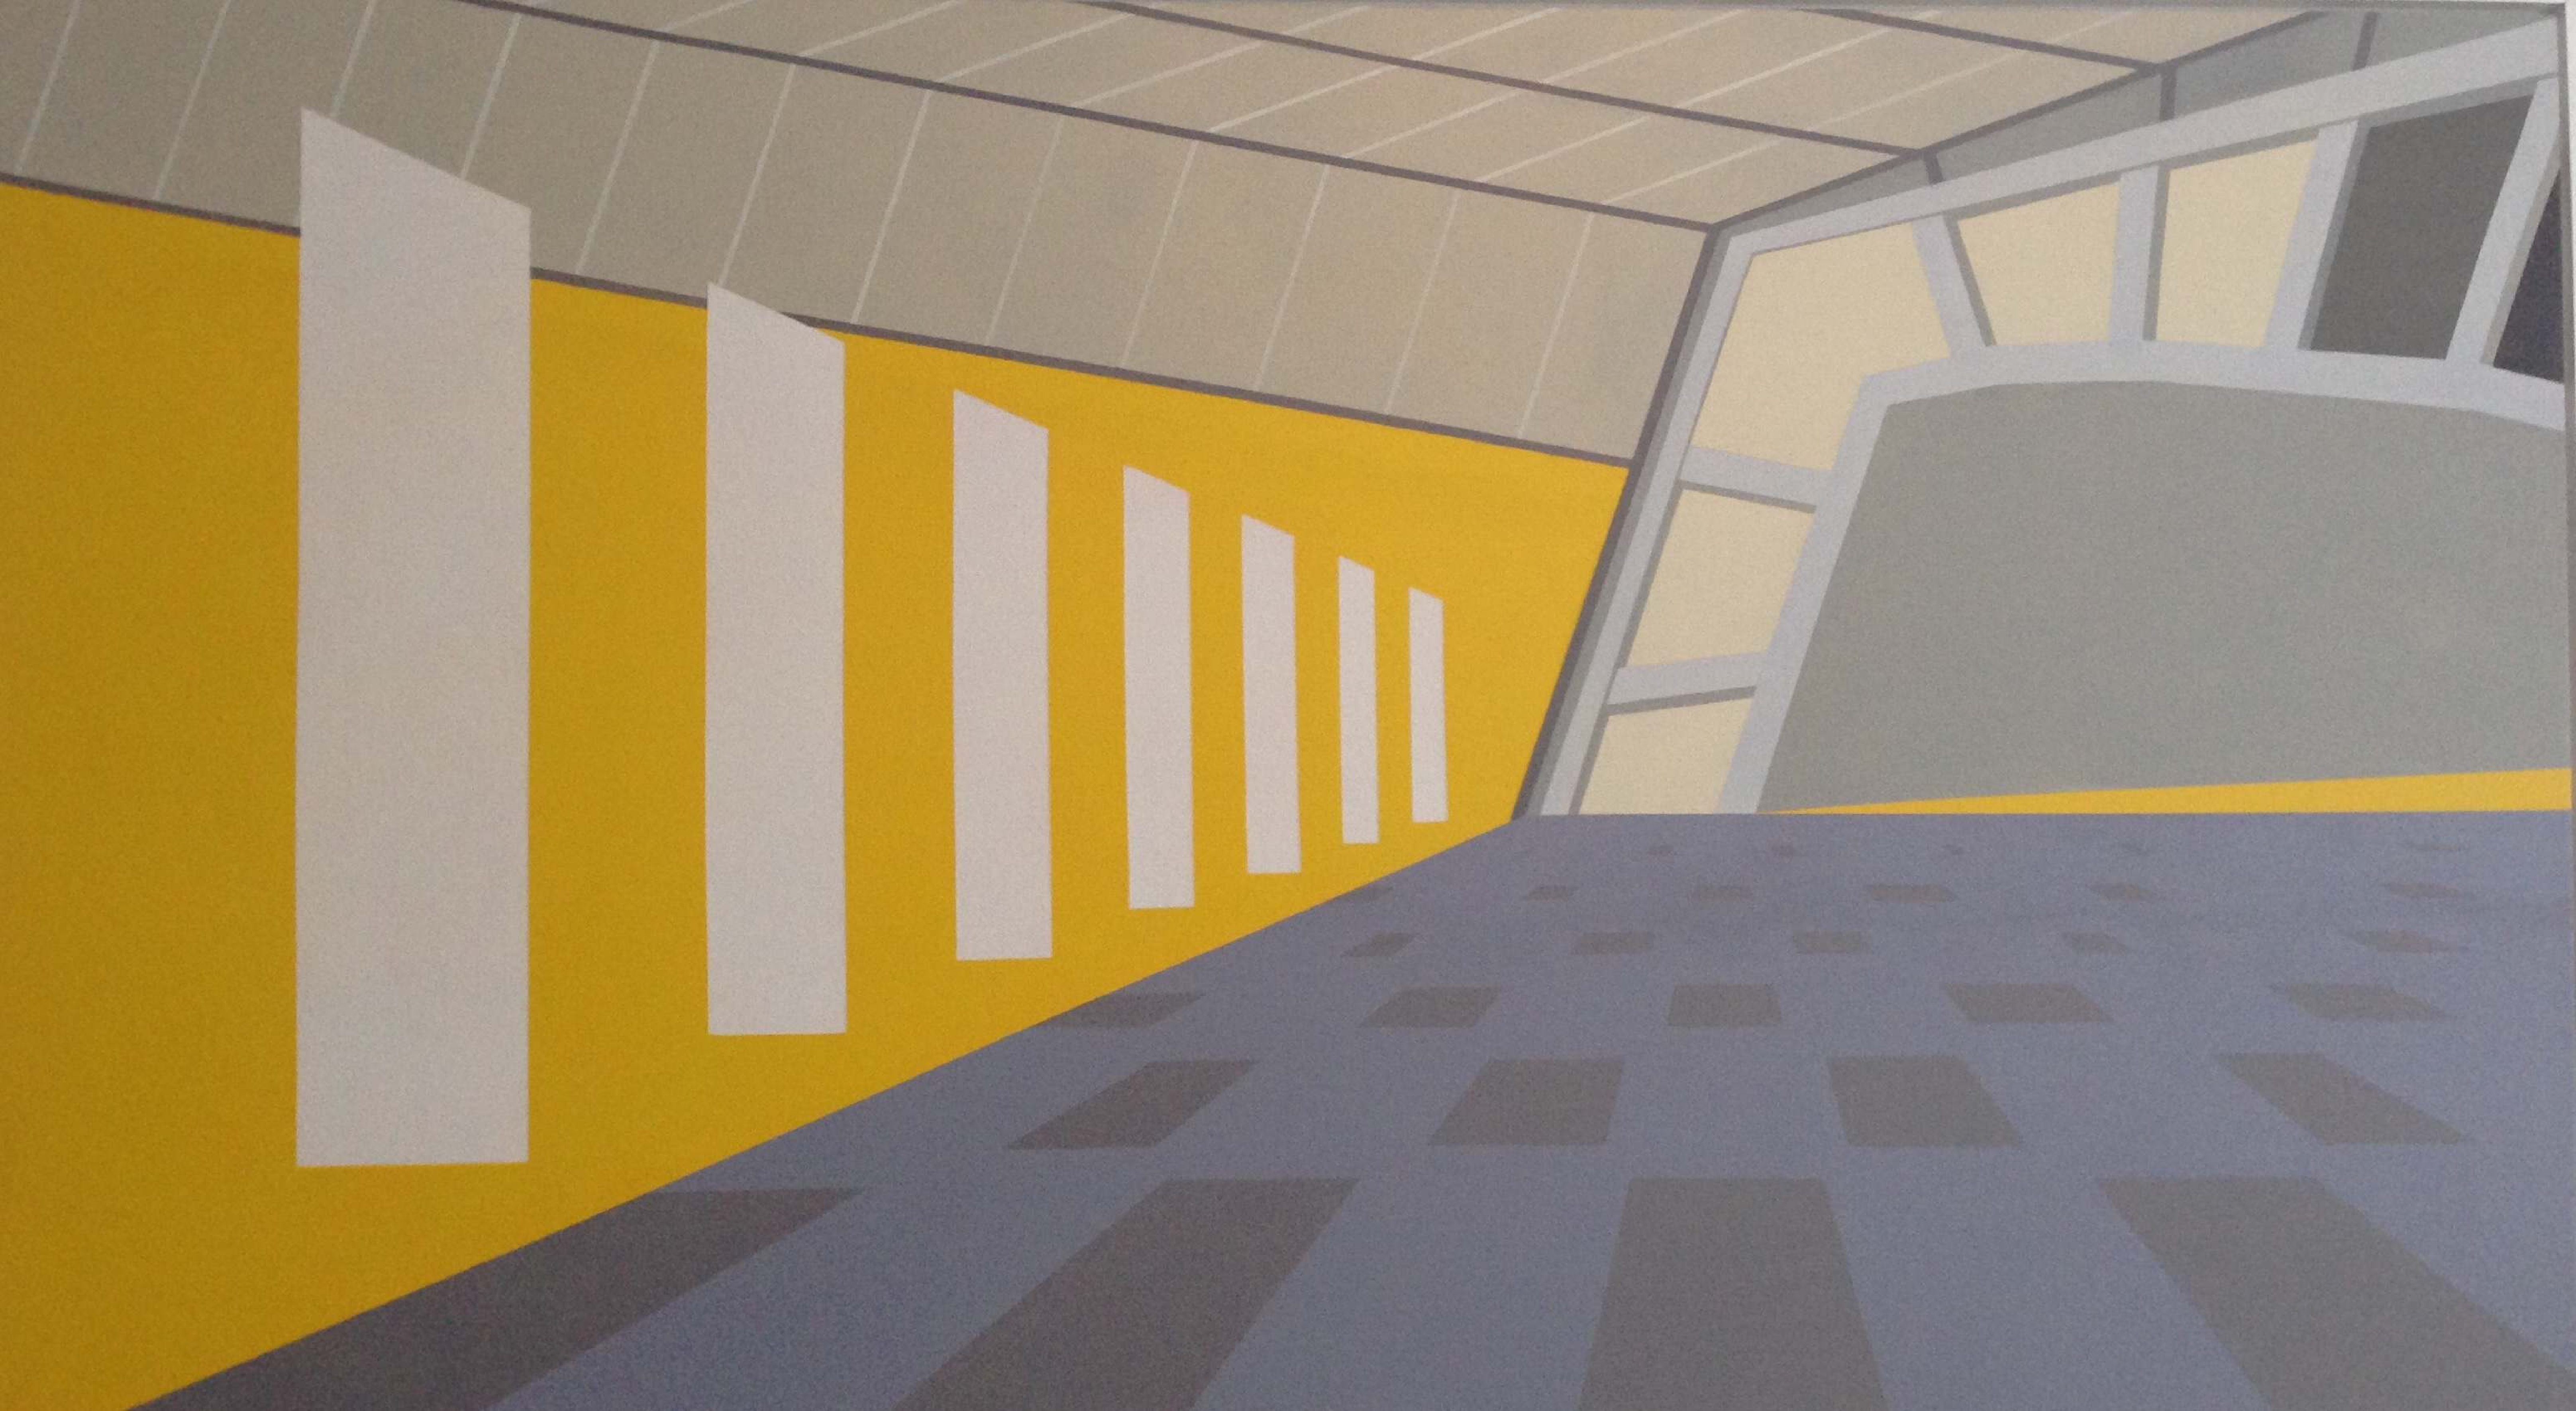
\includegraphics[width=4.73436in,height=2.54545in]{figuras/odette-gare-no-cinema.pdf.compressed.pdf}
  \figurenote{\series{Arena}. \acrilico. \artsize{80 x 144}. \photoreg.}
\end{figure}

Nesta dissertação, um dos alicerces da metodologia de investigação é a
poética que está sendo construída no ateliê da FBAUP, a partir de 2019,
utilizando-se da conjugação de vivências em dois meios distintos,
cinema e pintura, que se desdobram até hoje em muitos estudos sobre
estratégias processuais e cor. Portanto, peço licença pelo
desdobramento de tantas ideias ao longo do texto, demandadas pela
prática e pelo próprio fazer da pintura, que se constrói juntamente com
a escrita.

No \cref{cap1-contexto-relacao-cinema-pintura} abordamos o contexto
histórico das vanguardas europeias da pintura relacionadas aos
primeiros filmes. Na sequência fazemos uma revisão de textos de autores
dos nossos tempos, como \textcite{aumont2004olho,gardies2019espaco,sardo2017exercicio}
que emprestam suas reflexões teóricas relacionadas
a conceitos de movimento em espaços de suportes tradicionais da
pintura, do cinema e da arte contemporânea.

No \cref{cap2-impacto-evolucao-otica}, analisamos o impacto na arte da
evolução da óptica relacionada à lente dos dispositivos câmera e
projetor. Sobre o dispositivo no cinema, encontramos no texto de 
\textcite{parente2007cinema}, na publicação \emph{Estéticas do digital}, reflexões
pertinentes\footnote{Em \textcite[10]{parente2007cinema}, \enquote{O
		conceito de dispositivo tem uma história filosófica forte na obra dos
		grandes filósofos pós-estruturalistas, em particular Michel Foucault,
		Gilles Deleuze e Jean-François Lyotard. Para eles, o efeito que o
		dispositivo produz no corpo social se inscreve nas palavras, nas
		imagens, nos corpos, nos pensamentos, nos afetos. É por essa razão que
		Foucault fala de dispositivos de poder e de saber, Deleuze fala de
		dispositivo de produção de subjetividade e Lyotard de dispositivos
		pulsionais. Cada um deles faz uso deste conceito para analisar uma obra
		em que a questão do dispositivo é como um manifesto do seu pensamento.}%
}, mas por se tratar de um conceito de larga amplitude, no campo da
filosofia, que vai além dos objetivos de ordem processual e práticos
desta investigação, decidimos não avançar nesta direção. Por outro
lado, na mesma publicação, \textcite{viveiros2007espacos}, em suas
análises da pintura Flamenga, destaca um momento onde as técnicas
revolucionaram o modo de composição espacial, relacionando-as ao cinema
dos primeiros tempos e ao cinema digital. Tratamos da direção do olhar
e do movimento no espaço do ecrã e da tela da pintura através do filme
de Majewski, \emph{O moinho e a cruz}, que representa a obra
\emph{Cristo no calvário}, de Bruegel, o Velho. Consideramos ainda
análises sobre o movimento na arte, apontadas nos textos \emph{Vida das
	Formas}
\parencite{focillon1983vida} e \emph{Rubens and Leonardo on Motion:
	Figures, Inscriptions, and Texts} \parencite{barone2009rubens}.

O método por nós utilizado de projetar imagens sobre a tela da pintura
como instrumento para marcar e pensar a composição, nos levou a visitar
elementos operativos da construção do filme, e recorremos a
categorizações propostas por \textcite{block2021visual}, sobre a
estrutura da narrativa visual do cinema. Abordamos ainda na seção
\cref{cap2-impacto-evolucao-otica} a influência da cor na estrutura
cenográfica do cinema e métodos pictóricos para estabelecimento de
paletas diante da evolução teórica dos estudos da cor. Esclarecemos que
nosso objeto de pesquisa não contempla a pintura expandida e a pintura
digital, pois nosso interesse é tratar de processos cuja tradição da
tinta e do gesto sobre um suporte bidimensional se mantém a despeito do
uso de novas tecnologias.

Na seção \cref{cap3-narrativa-visual} objetivamos investigar como é feita a
seleção, pelos pintores, das referências que apoiarão seus projetos.
Analisamos os processos criativos desenvolvidos por duas pintoras
brasileiras que se destacam atualmente no cenário internacional da arte
contemporânea: Lucia Laguna (1941),~com suas estruturas de paisagem no
espaço urbano limitado pelo quadro e Cristina Canale (1961), com~uma
estética vinculada à moda e à cor.

Na seção \cref{cap4-entre-projeto-processo} apresento o trabalho plástico
desenvolvido no ateliê do mestrado, com o trajeto das experimentações
de processos e técnicas de pintura a óleo, realizadas durante o período
desta investigação. Por fim, vinculamos assuntos explorados nesta
dissertação, como por exemplo o do espaço profundo no cinema, ao
projeto expositivo pessoal intitulado \emph{Olhar do cinema}. Desta
forma esperamos, não só encontrar possíveis respostas para as questões
elencadas no início do texto, mas também propor alternativas e
contribuir com possibilidades de caminhos e escolhas processuais
alinhadas à poética de artistas que trabalham no âmbito da pintura e da
arte contemporânea.
